\documentclass[12pt,a4paper]{article}
\usepackage[margin=1in]{geometry}
\usepackage[moduleName=2612]{KautenjaDSP}
% import a debugging package to show the margin boxes
% \usepackage{showframe}
% set the graphics path to the img directory
\graphicspath{{img/}}

% algorithm2e stuff
% \SetKwInOut{Objects}{$\CKmatrix{O}$}
% \SetKwInOut{Weights}{$\CKvector{w}$}

\begin{document}
\titlePage{2612-Logo}{2612-Module}{KautenjaDSP}

% -------------------
% MARK: Overview
% -------------------

\section{Overview}

2612 is an emulation of the Yamaha YM2612 audio processing unit from the Sega Master System and Sega Genesis for VCV Rack. The YM2612 is a 4-operator FM synthesis chip with 6 voices of polyphony.

2612 provides the key features of the 2612 chip, namely,
\begin{itemize}
  \item \textbf{16-bit:} 8 bits better than the previous generation of chips!
  \item \textbf{6 Voice Polyphony:} 6 voices of polyphony with independent V/OCT and Gate inputs
  \item \textbf{4-Operator FM Synthesis:} Full control over the FM-synthesis parameters for each of the four operators including: envelopes, multiplier rate scale, tuning, and amplitude modulation
  \item \textbf{8 FM Algorithms:} 8 different arrangements of the four operators
  \item \textbf{Stereo Outputs:} Output from the left and right channels on the chip
\end{itemize}

% -------------------
% MARK: Panel Layout
% -------------------

\clearpage
\section{Panel Layout}

\begin{figure}[!htp]
\centering
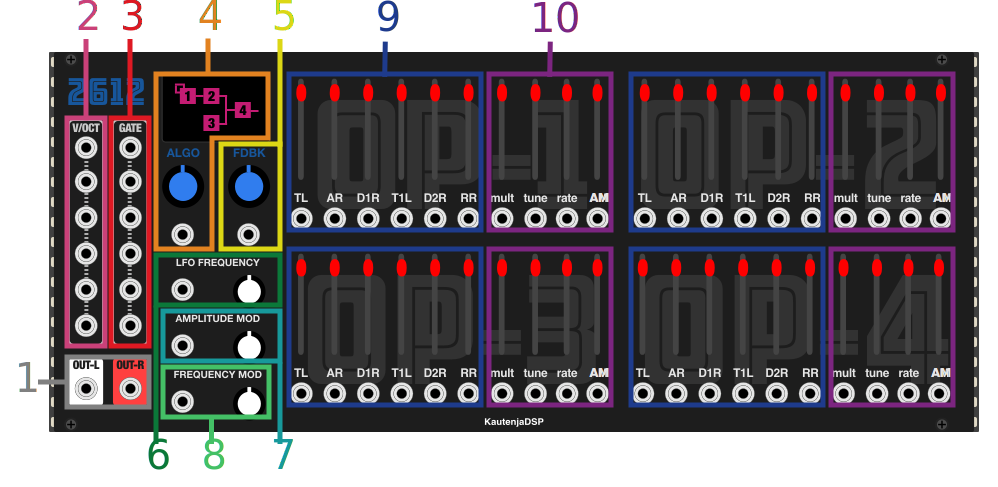
\includegraphics[width=\maxwidth{\textwidth}]{2612-Manual}
\end{figure}

% \begin{enumerate}
%   \item Coarse frequency control over the four oscillators.
%   \item $V$/Octave inputs for pulse1, pulse2, and triangle waveform generators.
%   \item linear CV frequency modulation for pulse1, pulse2, and triangle waveform generators.
%   \item Pulse width selector. Chooses between four duty cycles: $12.5\%$, $25\%$, $50\%$, and $75\%$.
%   \item CV LFSR gate, high at $2V$. Holds the LFSR generator as long as the input voltage is $>2V$.
%   \item Period of randomness $\in [0, 15]$ for the noise generator. See Table~\ref{tab:noise-periods} for a mapping from period to sample rate, frequency, and MIDI note.
%   \item Coarse amplitude control over the oscillators using the 4-bit amplifier. When no input is connected, the slider controls the level from $0\%$ to $100\%$. When an input is connected, the slider acts as an attenuator.
%   \item Channel outputs, ${\approx}10V_{pp}$.
% \end{enumerate}

% -------------------
% MARK: References
% -------------------

\clearpage
\renewcommand\refname{References \& Acknowledgments}
\nocite{*}
\bibliographystyle{apalike}
\bibliography{references}

\end{document}
